\chapter{Testes e Resultados}
\label{ch::testes}

\section{Introdução}
\label{sec::testes:intro}

Bla bla inicial\ldots


\section{Secções?}
A analisar\ldots


\begin{figure}[!htbp]
	\centering
	
\includegraphics[width=.8\textwidth]{home}
	\caption[Ecrã inicial da aplicação]{Ecrã inicial da aplicação \theapp.}
	\label{fig::home}
\end{figure}

\begin{figure}[!htbp]
	\centering
	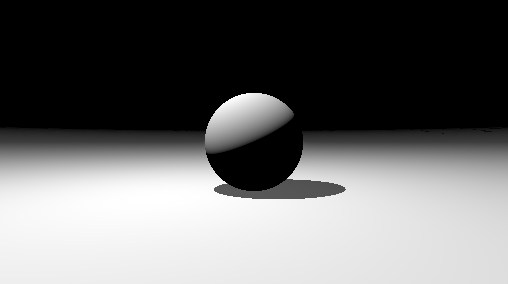
\includegraphics[width=.8\textwidth]{spheresphere}
	\caption[Teste do algoritmo de \textit{sphere tracing}]{Teste do algoritmo de \textit{sphere tracing} no \textit{website} \url{shadertoy.com} de uma esfera e um plano.}.
	\label{fig::spheresphere}
\end{figure}

\begin{figure}[!htbp]
	\centering
	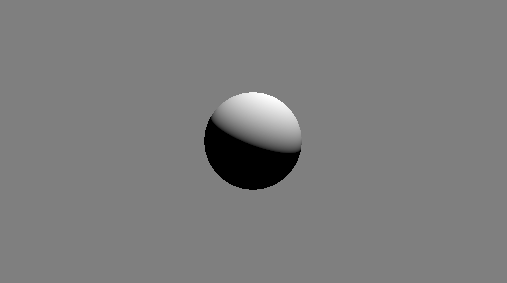
\includegraphics[width=.8\textwidth]{ashalgosphere}
	\caption[Teste do algoritmo naïve]{Teste do algoritmo naïve no \textit{website} \url{shadertoy.com} de uma esfera.}
	\label{fig::ashalgosphere}
\end{figure}

\begin{figure}[!htbp]
	\centering
	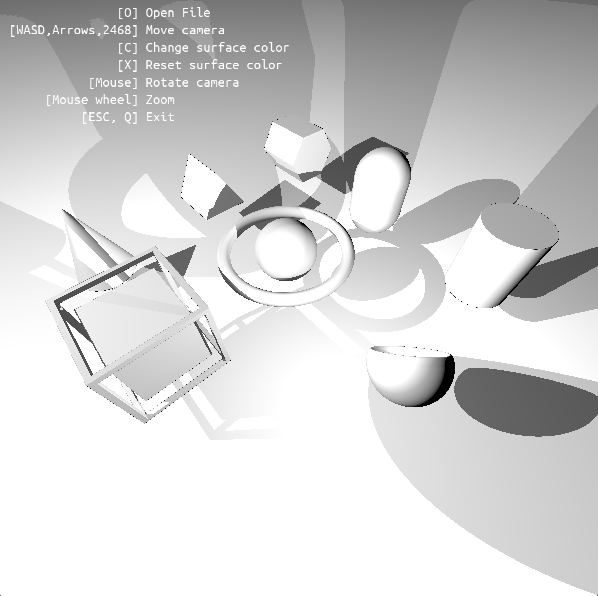
\includegraphics[width=.8\textwidth]{sphereoriginal}
	\caption[Nove objetos com \textit{sphere tracing} no \theapp]{Renderização de nove objetos no \theapp~usando o algoritmo de \textit{sphere tracing}.}
	\label{fig::sphereoriginal}
\end{figure}

\begin{figure}[!htbp]
	\centering
	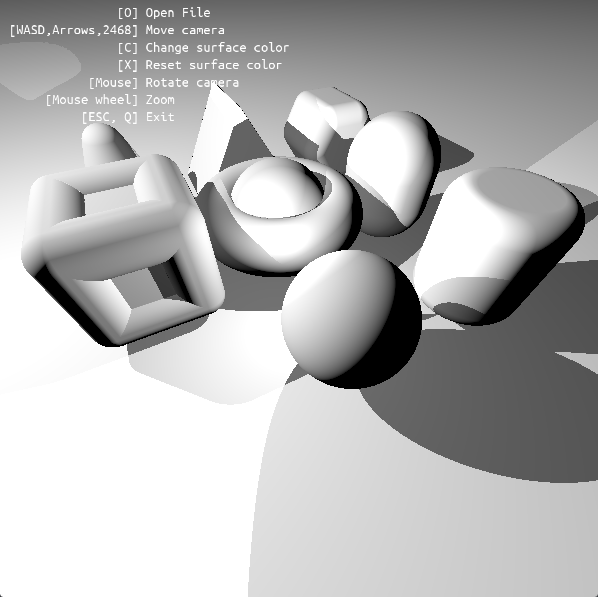
\includegraphics[width=.8\textwidth]{spheresmooth}
	\caption[Nove objetos com \textit{sphere tracing} e suavização no \theapp]{Renderização de nove objetos no \theapp~usando o algoritmo de \textit{sphere tracing} com um fator de suavização $s$ dependente do tempo de execução $t$, em particular $s = \cos(t)$.}
	\label{fig::spheresmooth}
\end{figure}

\begin{figure}[!htbp]
	\centering
	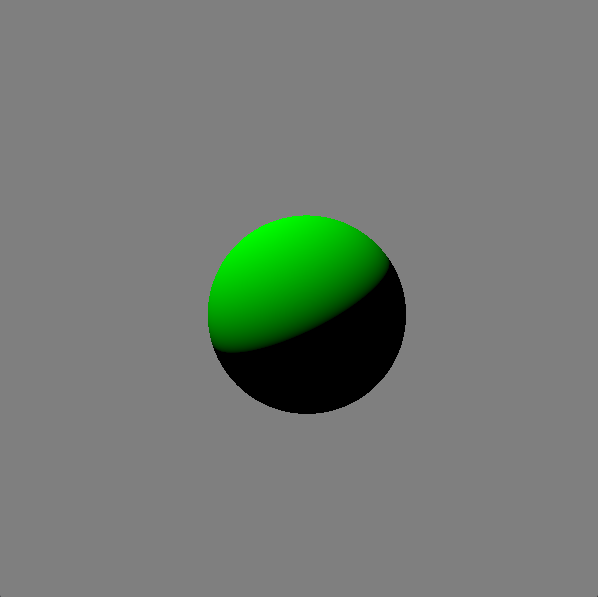
\includegraphics[width=.8\textwidth]{calcglsphere}
	\caption[Esfera no \theapp~com algoritmo naïve]{Esfera renderizada no \theapp, em fase inicial de testes, com o algoritmo naïve.}
	\label{fig::calcglsphere}
\end{figure}

\begin{figure}[!htbp]
	\centering
	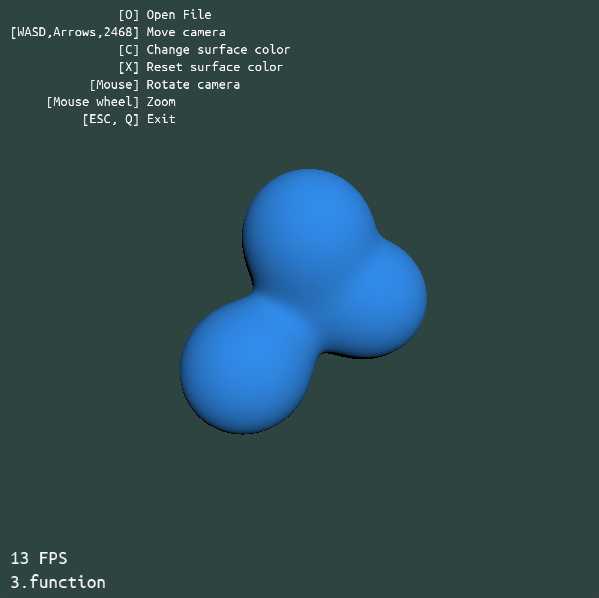
\includegraphics[width=.8\textwidth]{calcglpisurf}
	\caption[Superfície $\Pi$ no \theapp~com algoritmo naïve]{Superfície $\Pi$ renderizada no \theapp~com algoritmo naïve.}
	\label{fig::calcglpisurf}
\end{figure}

\begin{figure}[!htbp]
	\centering
	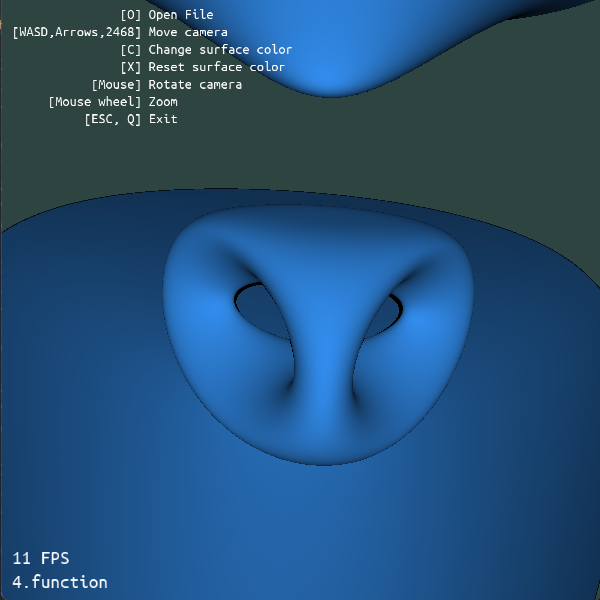
\includegraphics[width=.8\textwidth]{calcglgenus}
	\caption[\textit{Genus} no \theapp~com algoritmo naïve]{\textit{Genus} renderizado no \theapp~com algoritmo naïve.}
	\label{fig::calcglgenus}
\end{figure}


\section{Conclusões}
\label{sec::testes:conc}

\ldots Whiskas Saquetas.
